The previous chapters focused on using camera models to identify the relationship between points in a 3D scene and their projections onto the camera image, as well as how to leverage those models to reconstruct 3D scene structure from 2D images. 
Alternatively, this chapter begins to look at methods for extracting other types of information through \textit{image processing}, for example to answer the question ``what object am I seeing?'' rather than ``how far away is this object?''.
Extracting this type of visual content from raw images is important for mobile robots to be able to intelligently interpret their surroundings. In fact, it can have a major impact on the ability of the robot to perform several tasks including localization and mapping or decision making. This chapter focuses on some of the more commonly used tools in image processing including image filtering, feature detection, and feature description\cite{SiegwartNourbakhshEtAl2011}\cite{Moravec1977}.

\notessection{Image Processing}
Image processing is a form of signal processing where the input signal is an image (such as a photo or a video) and the output is either an image or a set of parameters associated with the image. While a large number of image processing techniques exist, this chapter focuses on some of the more fundamental methods that are relevant for robotics. In particular, these methods will be related to image filtering, feature detection, and feature description\footnote{The software library OpenCV implements a number of useful image filtering algorithms: \url{https://docs.opencv.org}.}.

In the following methods, grayscale images are treated as functions $I$: $[a,b]\times[c,d] \rightarrow [0,L]$, where $I(x,y)$ represents the grayscale pixel intensity at $(x,y)$. 
For a color image, $I$ is a vector valued function with three components, one each for the red, green, and blue color channels of the image.

\subsection{Image Filtering}
Image filtering is one of the principal tasks in image processing. The terminology ``filter'' comes from frequency domain signal processing and refers to the process of accepting or rejecting certain frequency components of a signal (e.g. eliminating high-frequency noise).

Perhaps the most common type of image filtering is \textit{spatial filtering}.
The basic principle of spatial filtering is that a particular pixel is modified in the filtered image based only on the pixels in the immediate spatial neighborhood (see Figure \ref{fig:spatial_filter_concept_fig}). To be more specific, a spatial filter for an image $I(x,y)$ consists of:
\begin{enumerate}
    \item A neighborhood $S_{xy}$ of pixels around a particular point $(x,y)$ under examination, typically rectangular.
    \item A predefined operation $F$ that is performed on the image pixels encompassed by the neighborhood $S_{xy}$.
\end{enumerate}
Once the operation $F$ has been applied to all pixels $(x,y)$ in the image $I$ a new image $I'(x,y)$ is defined.
\begin{figure}[ht]
  \centering
  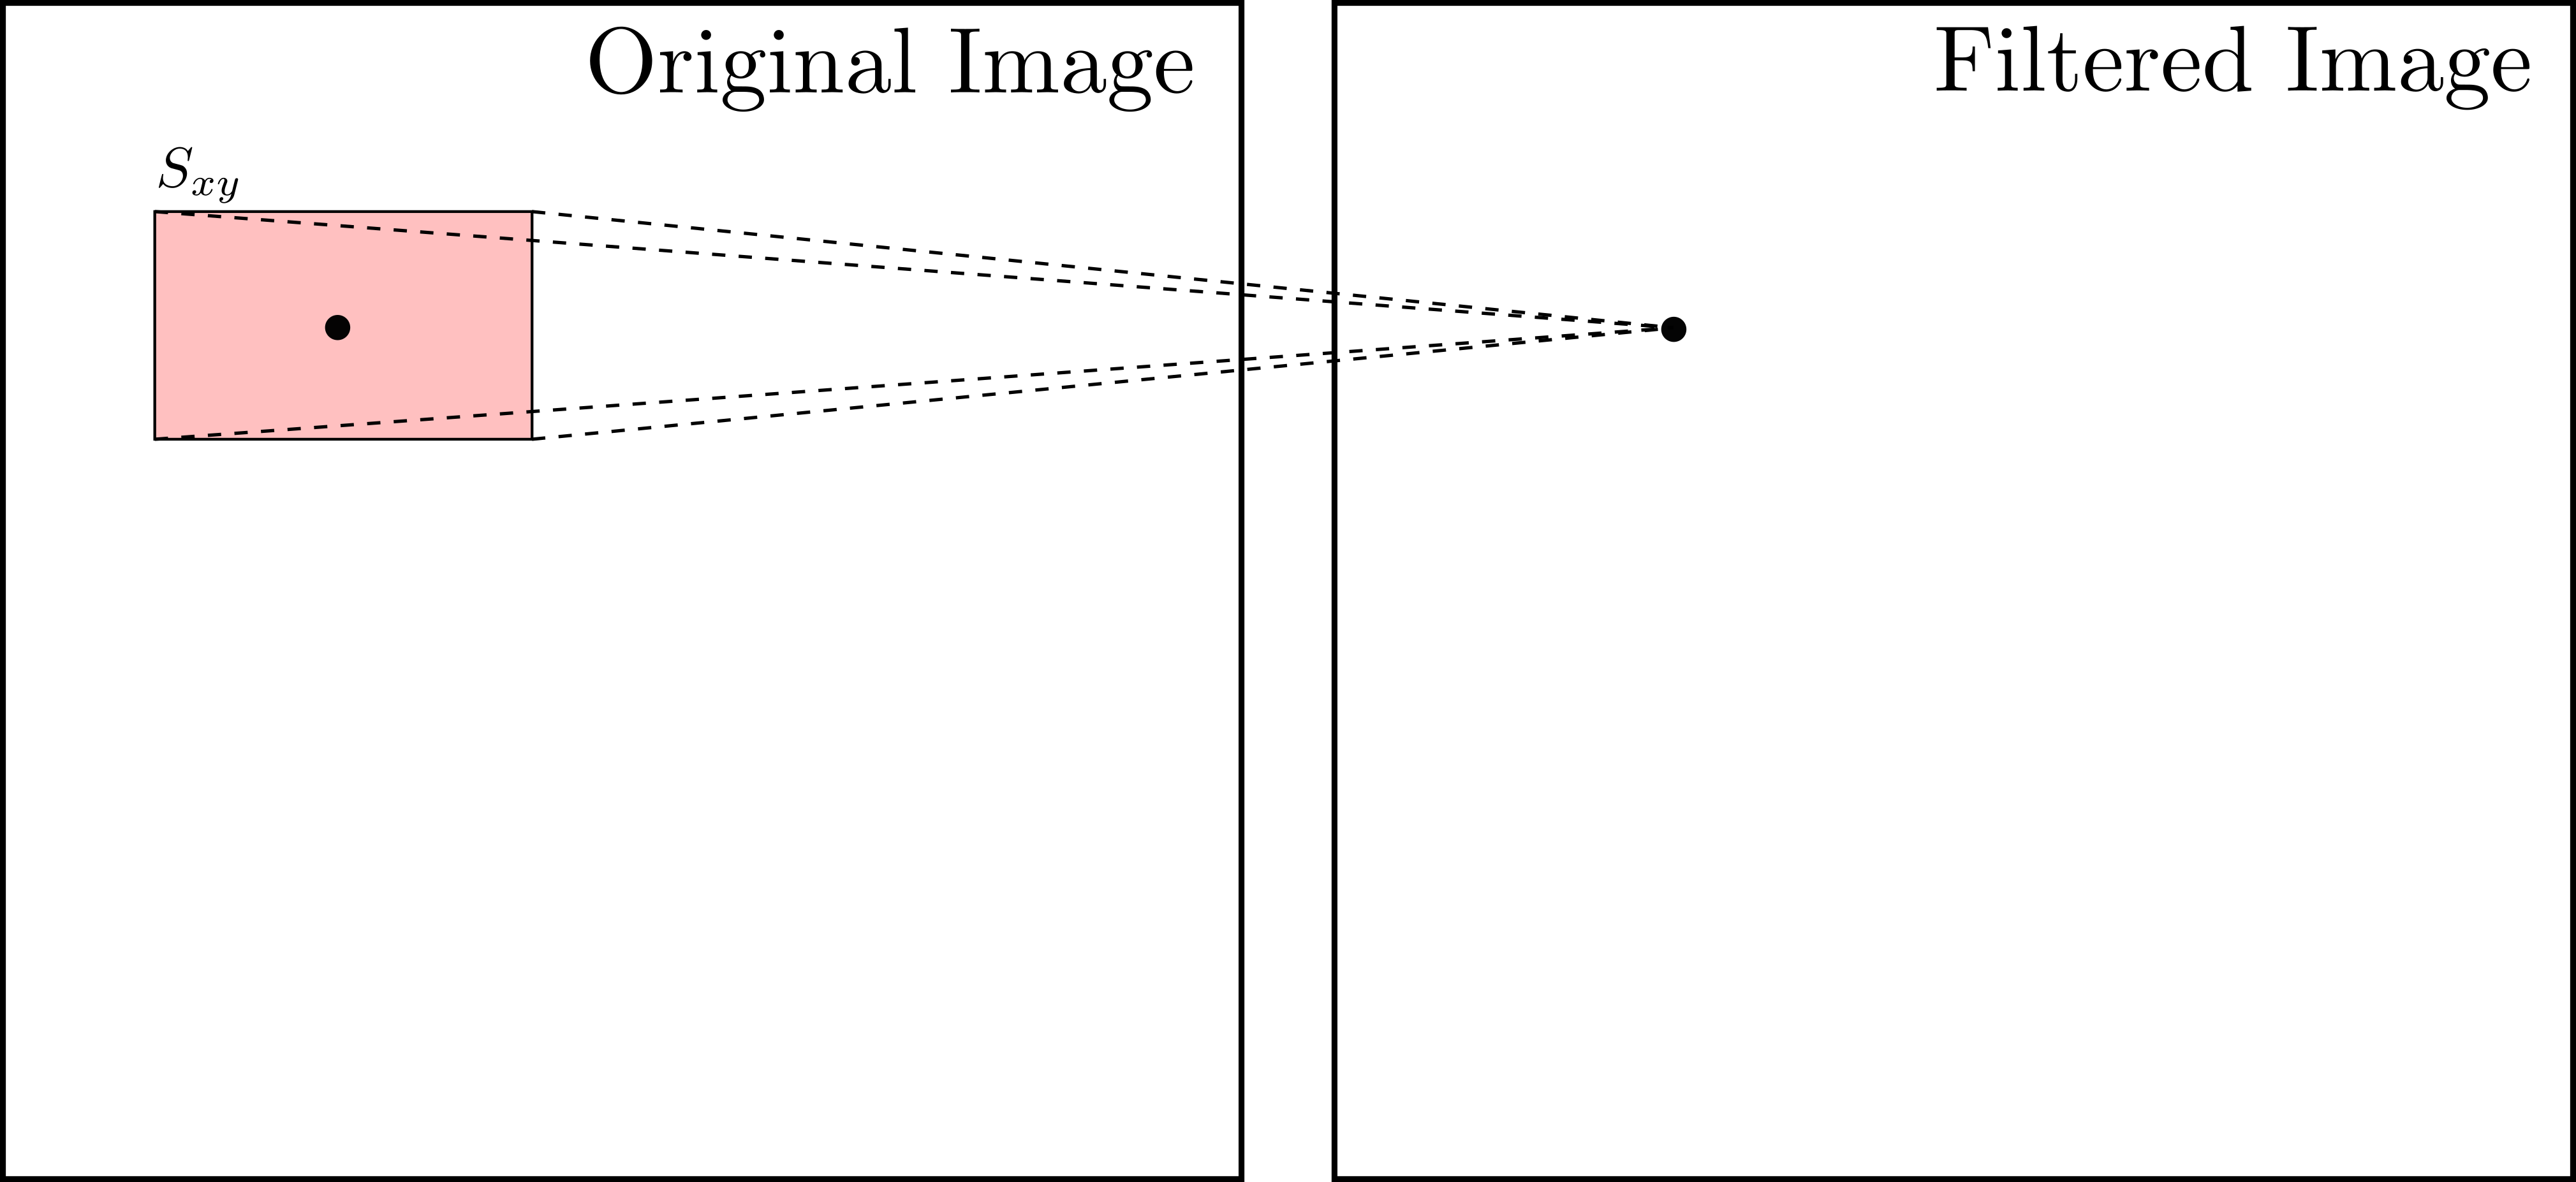
\includegraphics[width=.75\textwidth]{tex/figs/ch10_figs/spatialfiltering.png}
    \caption{Illustration of the concept of spatial filtering. The spatial filter operates on a neighborhood $S_{xy}$ of each point in the original image to produce a new pixel in the filtered image.}
    \label{fig:spatial_filter_concept_fig}
\end{figure}

In general filters can be linear or nonlinear, but many of the most fundamental filters are linear and can be expressed mathematically as:
\begin{equation}
  \label{eq:correlation}
    I'(x,y) = F \circ I = \sum_{i=-N}^N \sum_{j=-M}^M F(i,j)I(x+i,y+j),
\end{equation}
where $N$ and $M$ are integers that define the width and height of a rectangular neighborhood $S_{xy}$. Based on the size of this neighborhood, it is said that this filter is of size $(2N+1) \times (2M+1)$. Additionally, the filter operation $F$ is usually called a \textit{mask} or \textit{kernel}. Broadly speaking, filters expressed by \eqref{eq:correlation} are referred to as \textit{correlation filters}.

Another type of linear filters that are commonly used are referred to as \textit{convolution} filters. Convolution filters are similar to correlation filters but use reverse image indices (in fact correlation and convolution filters are identical when the filter mask is symmetric in both the horizontal and vertical directions). In particular, these filters are expressed mathematically as:
\begin{equation}
  \label{eq:convolution}
    I'(x,y) = F \ast I = \sum_{i=-N}^N \sum_{j=-M}^M F(i,j)I(x-i,y-j).
\end{equation}
Convolution filters are associative, meaning that for two different filter masks $F$ and $G$ it is true that $F*(G*I) = (F*G)*I$. One example of how the associative property is useful is for smoothing an image \textit{before} taking applying a differentiation filter. Suppose the mask $F$ implemented a derivative filter and $G$ implemented a smoothing filter, then sequentially applying these filters would result in $F*(G*I)$. However, because of the associative property the masks can be convolved together \textit{first} such that only one filter needs to be applied to the image (i.e. $(F*G)*I$).

Note that in both the correlation and convolution filters the boundaries of the image need some special care because of the width and height of the mask. For example, Figure \ref{fig:nopaddingexample} shows how the filtered image is smaller than the original due to the width and height of the mask. Some possible options to handle this include padding the image, cropping it, extending it, or wrapping it. However, as images are generally quite large the exact approach likely won't vary the final result significantly.
\begin{figure}[ht]
  \centering
  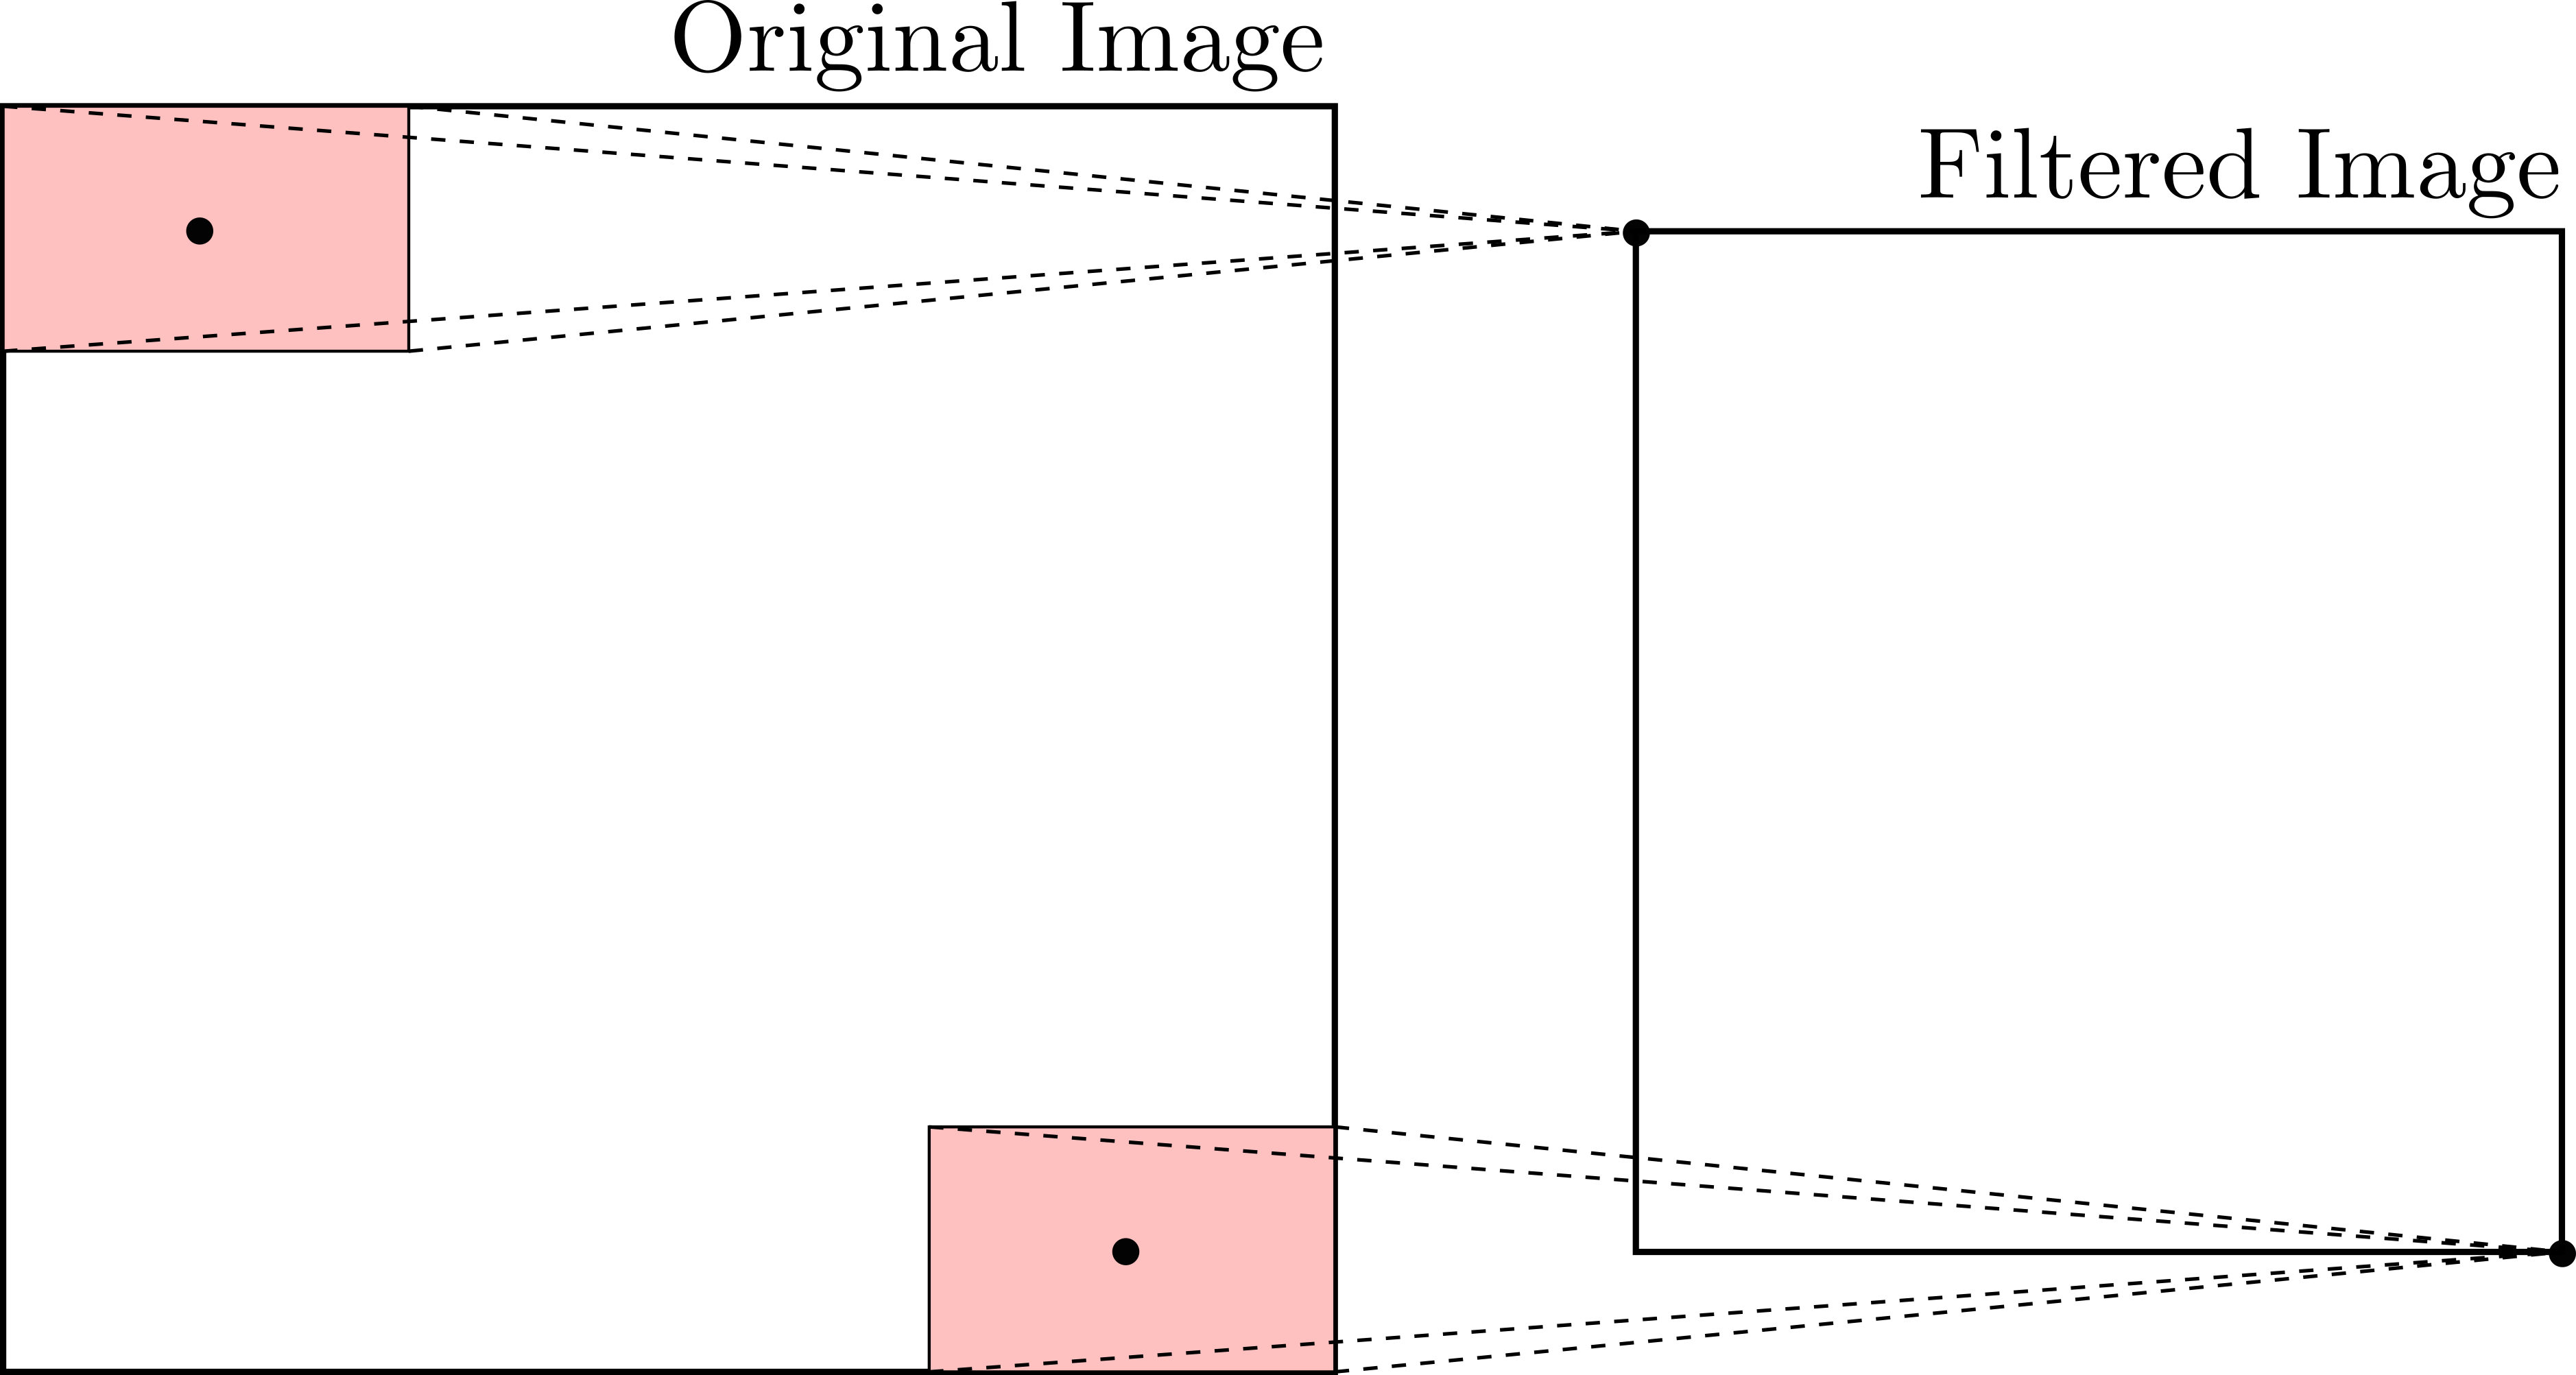
\includegraphics[width=.65\textwidth]{tex/figs/ch10_figs/centerfilter_nopadding.png}
    \caption{Due to the width and height of the mask, the filtered image may be smaller than the original. However this can be fixed with several techniques, such as padding.}
    \label{fig:nopaddingexample}
\end{figure}

\begin{example}[Practical Considerations for Image Filtering] \label{ex:padding}
\theoremstyle{definition}
Implementation of correlation and convolution filters typically leverages some additional ``tricks'' to make things easier to implement. In this example two such tricks will be introduced: zero-padding and a change in indexing. 

First, to more simply accommodate varying sizes of filters (including even and odd sized filters) the indexing is often changed such that the coordinate of interest is associated with the top-left element in the window rather than the center. In particular, for a correlation filter this would correspond to:
\begin{equation}
  \label{eq:correlation_newindex}
    I'(x,y) = F \circ I = \sum_{i=1}^K \sum_{j=1}^L F(x,y)I(x+i-1,y+j-1),
\end{equation}
where $K$ and $L$ are integers that define the width and height of the filter and the pixel $(x,y)$ is at row $x$ and column $y$. However, note that with this formulation the output image $I'$ will be shifted up and to the left. To see this consider the pixel at $x=1$ and $y=1$ in the new image $I'$, which would correspond to the top-left pixel $I'$. This new pixel value is generated by applying the filter $F$ over the pixels in the original image $I$ at rows $\{1,\dots,K\}$ and columns $\{1,\dots,L\}$ (which is not centered at $(1,1)$ in the original image $I$). Therefore it will appear as if the image has been shifted! But in practice this isn't an issue as long as you always index with respect to the top-left corner. An example of top-left indexing is shown in Figure \ref{fig:topleftfilter}
\begin{figure}[ht]
  \centering
  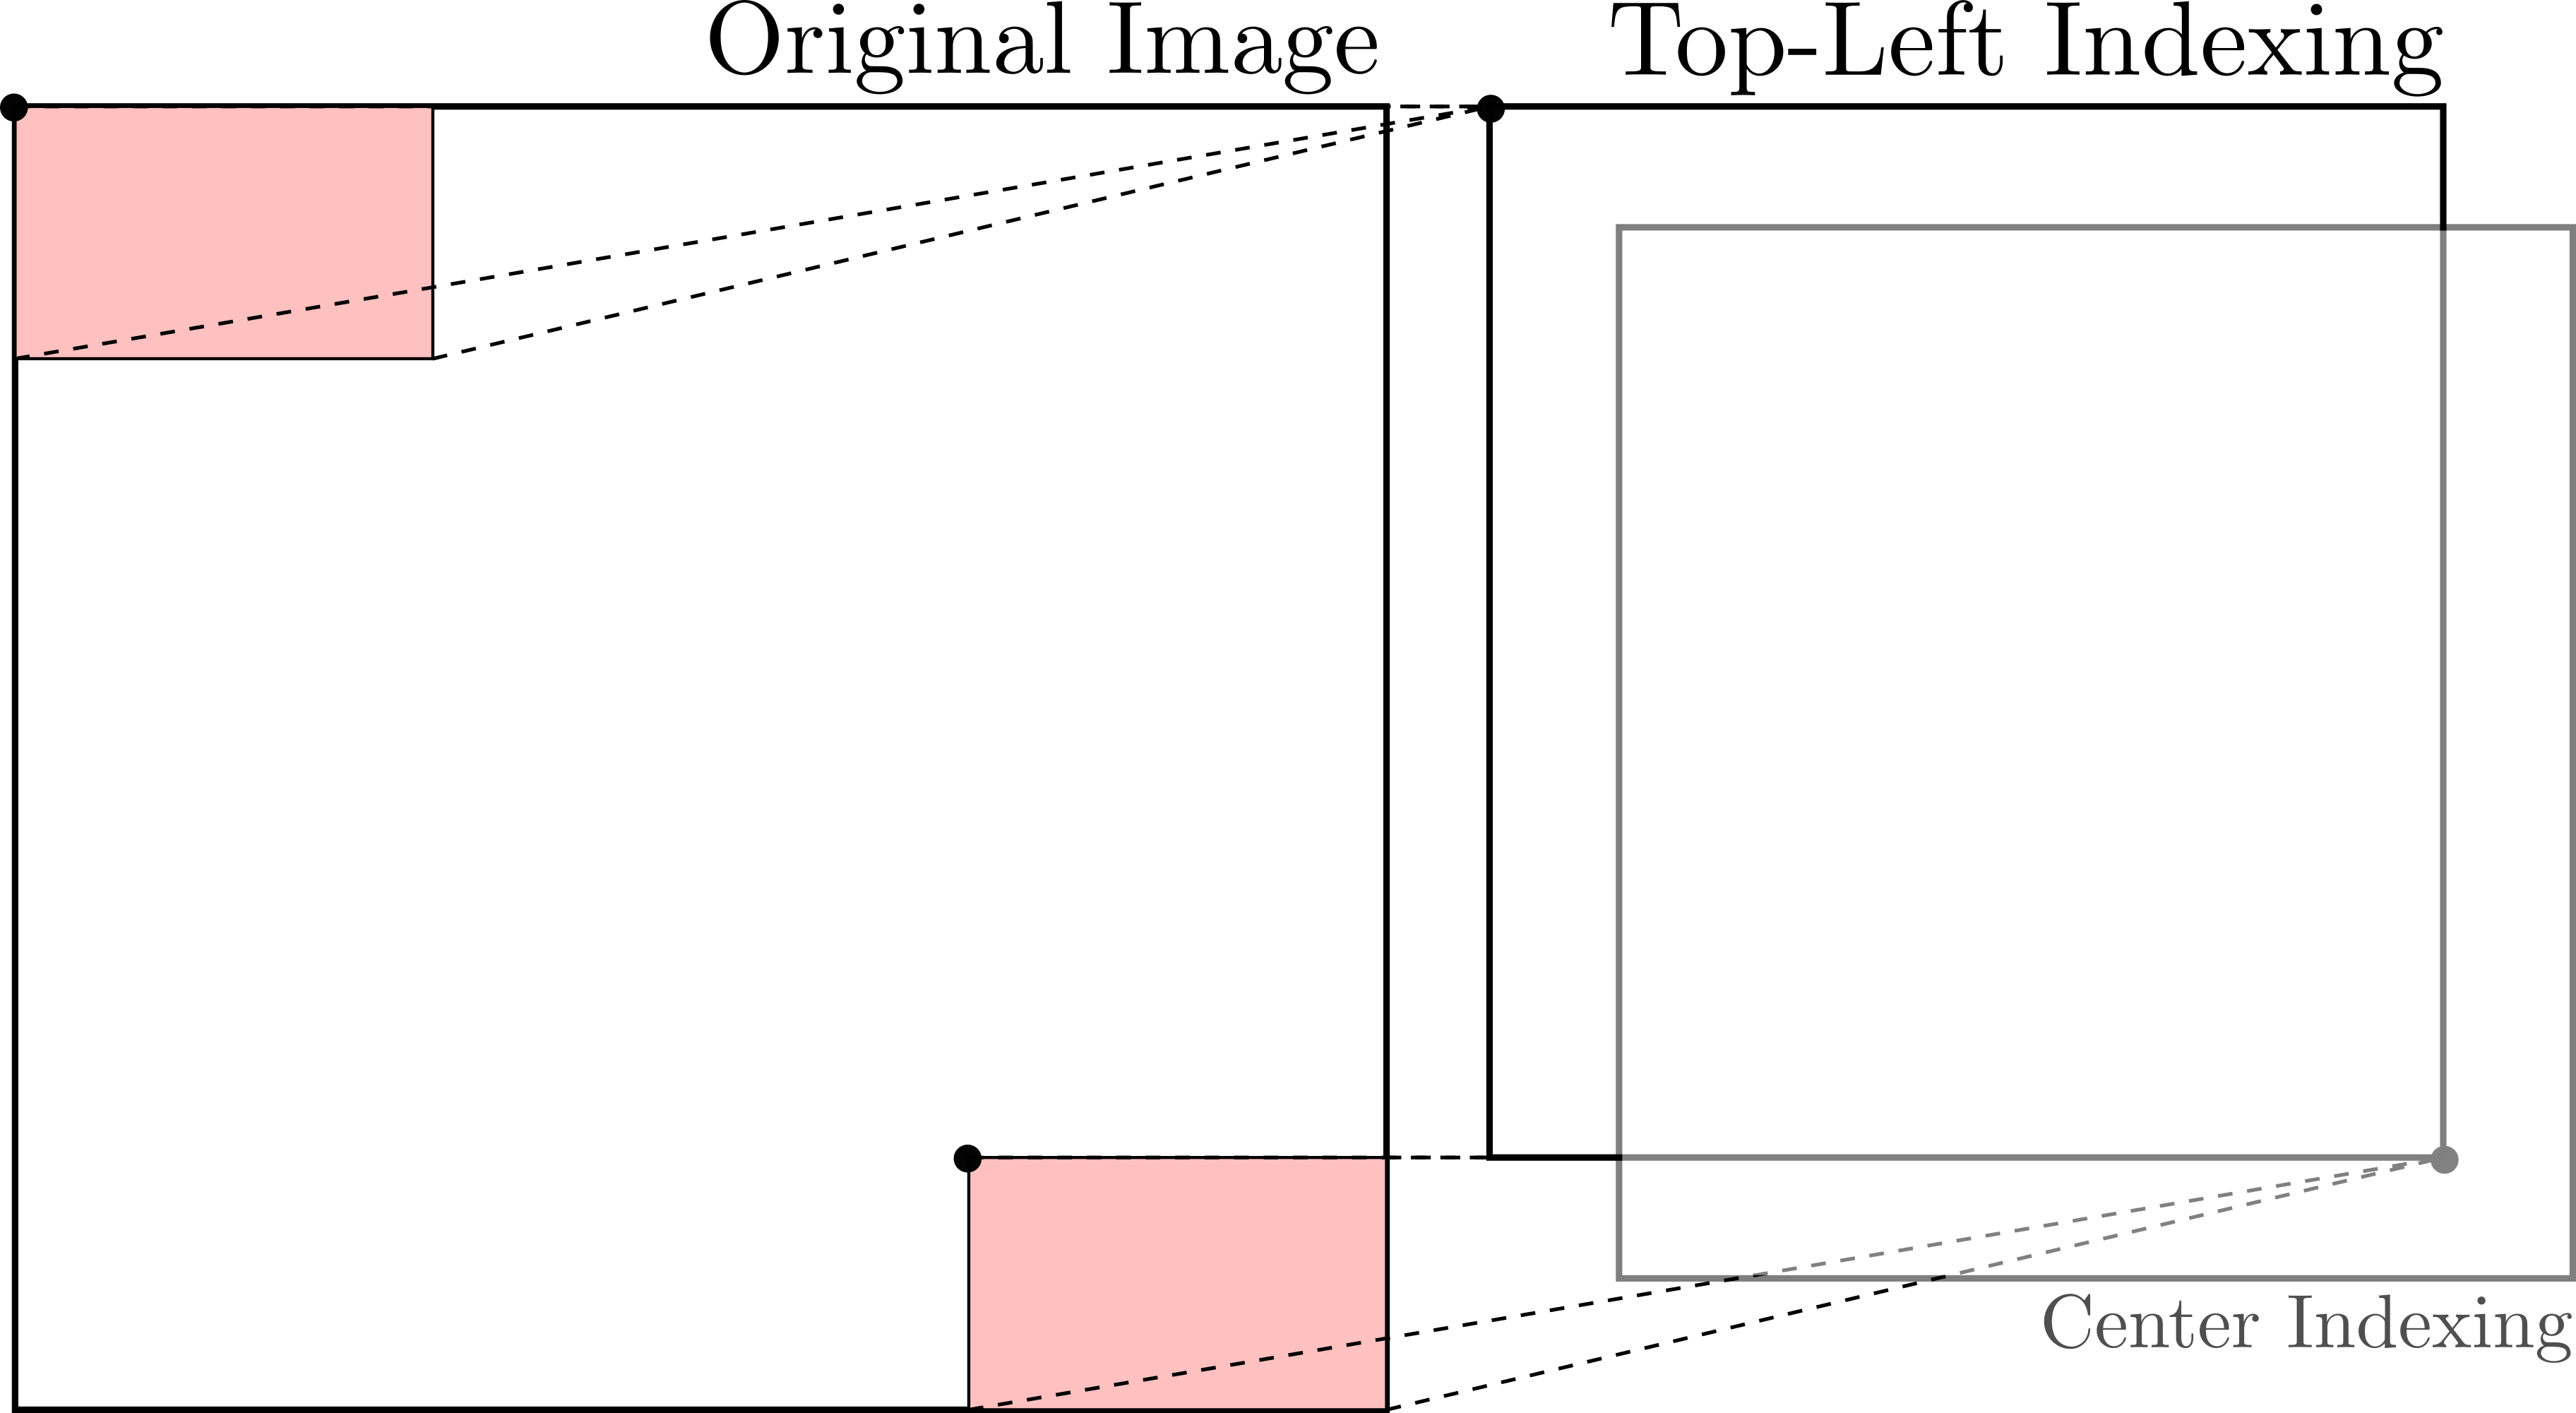
\includegraphics[width=.65\textwidth]{tex/figs/ch10_figs/topleftfilter_nopadding.png}
    \caption{Top-left indexing is typically easier to implement than center indexing. Notice that when top-left indexing, it appears as if the filtered image has shifted with respect to when center indexing is used.}
    \label{fig:topleftfilter}
\end{figure}

Zero-padding (also commonly referred to as \textit{same padding}) is another simple trick that can be used to ensure that the output filtered image $I'$ has the same dimension as the input image $I$. In this approach the left and right boundaries of the image are \textit{each} padded by $\lfloor K/2 \rfloor$ columns of zeros, and the top and bottom boundaries are padded by $\lfloor L/2 \rfloor$ rows of zeros ($\lfloor \cdot \rfloor$ denotes the ``floor'' operation). For example the image:
\begin{equation*}
I = \begin{bmatrix}
    1 & 2 & 3 \\
    4 & 5 & 6 \\
    7 & 8 & 9 \\
    \end{bmatrix},
\end{equation*}
would become
\begin{equation*}
I_\text{padded} = \begin{bmatrix}
    0 & 0 & 0 & 0 & 0 \\
    0 & 1 & 2 & 3 & 0 \\
    0 & 4 & 5 & 6 & 0 \\
    0 & 7 & 8 & 9 & 0 \\
    0 & 0 & 0 & 0 & 0 \\
    \end{bmatrix},
\end{equation*}
for filters $F \in \R^{3\times 3}$, $F \in \R^{2 \times 2}$, $F \in \R^{2 \times 3}$ and $F \in \R^{3 \times 2}$. When using this padding rule with the correlation filter \eqref{eq:correlation_newindex} and a filter $F$ with $K = 2,3$ and $L= 2,3$, the new image $I'$ can be defined for values $x \in \{1,2,3\}$ and $y \in \{1,2,3\}$, resulting in $I'$ being the same dimension as the original image $I$. The use of padding (along with top-left indexing) is also shown graphically in Figure \ref{fig:paddingfilter}
\begin{figure}[ht]
  \centering
  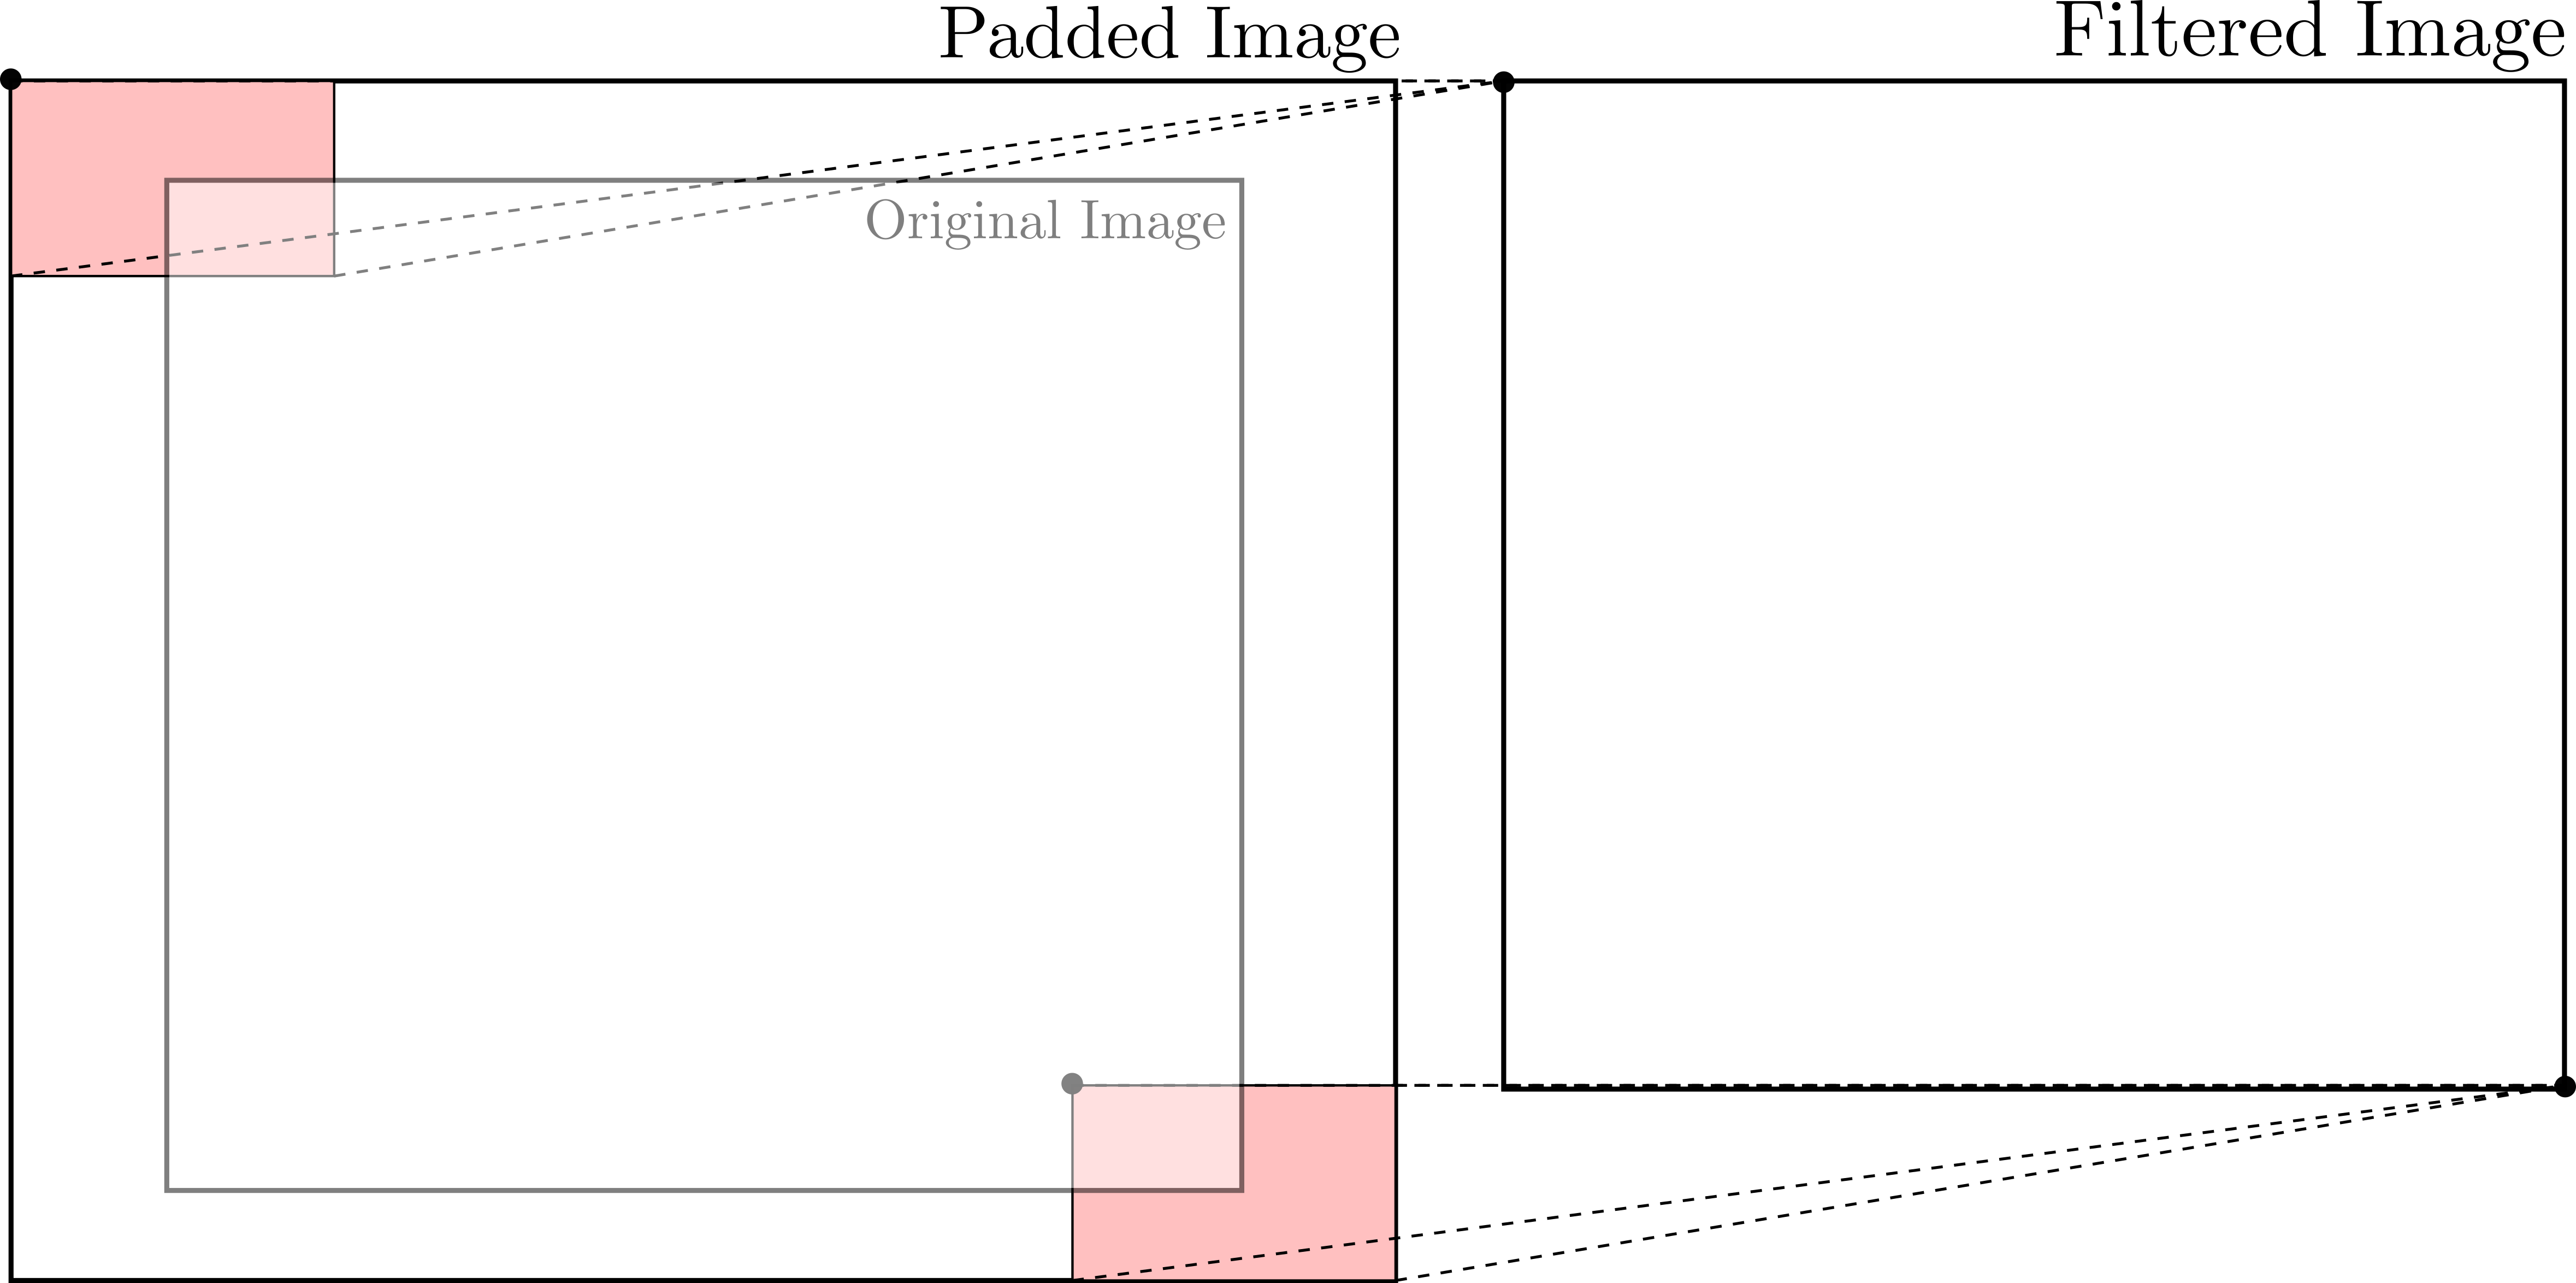
\includegraphics[width=.7\textwidth]{tex/figs/ch10_figs/topleftfilter_padding.png}
    \caption{Image padding is a commonly used technique to ensure that the size of the filtered image is the same size as the original.}
    \label{fig:paddingfilter}
\end{figure}
\end{example}


\subsubsection{Moving Average Filter}
The moving average filter returns the average of pixels in the mask, which achieves a smoothing effect (i.e. removes sharp features in the image). For example, a moving average filter with a normalized $3 \times 3$ mask is defined with the operation $F$ in \eqref{eq:correlation} chosen as:
\begin{equation*}
    F = \frac{1}{9}\begin{bmatrix}
    1 & 1 & 1 \\
    1 & 1 & 1 \\
    1 & 1 & 1 \\
    \end{bmatrix}.
\end{equation*}
Note that due to symmetry of the mask, the correlation \eqref{eq:correlation} and convolution \eqref{eq:convolution} filters will be identical. Additionally, the normalization is used to maintain the overall brightness of the image.

\subsubsection{Gaussian Smoothing Filter}
Gaussian smoothing filters are similar to the moving average filer, but instead of weighting all of the pixels evenly they are weighted by the Gaussian function:
\begin{equation*}
G_\sigma(x,y) = \frac{1}{2\pi\sigma^2} \exp \bigg(-\frac{x^2 + y^2}{2\sigma^2} \bigg).
\end{equation*}
This function is used to obtain the mask operation $F$ by sampling the function about the center pixel (i.e. for the center pixel with $i=j=0$ in \eqref{eq:correlation}, sample $G_\sigma(0,0)$). For example, for a normalized $3\times3$ mask with $\sigma$ = 0.85 this filter is approximately defined by:
\begin{equation*}
F = \frac{1}{16}
\begin{bmatrix}
1 & 2 & 1\\
2 & 4 & 2\\
1 & 2 & 1
\end{bmatrix}.
\end{equation*}
Like the moving average filter, this filter mask is symmetric and therefore yields identical results with respect to the correlation \eqref{eq:correlation} or convolution \eqref{eq:convolution} filters. The advantage of the Gaussian filter is that it provides more weight to the neighboring pixels that are closer.  An example of this filter is shown in Figure \ref{fig:gaussianfilter}.
\begin{figure}[ht]
  \centering
  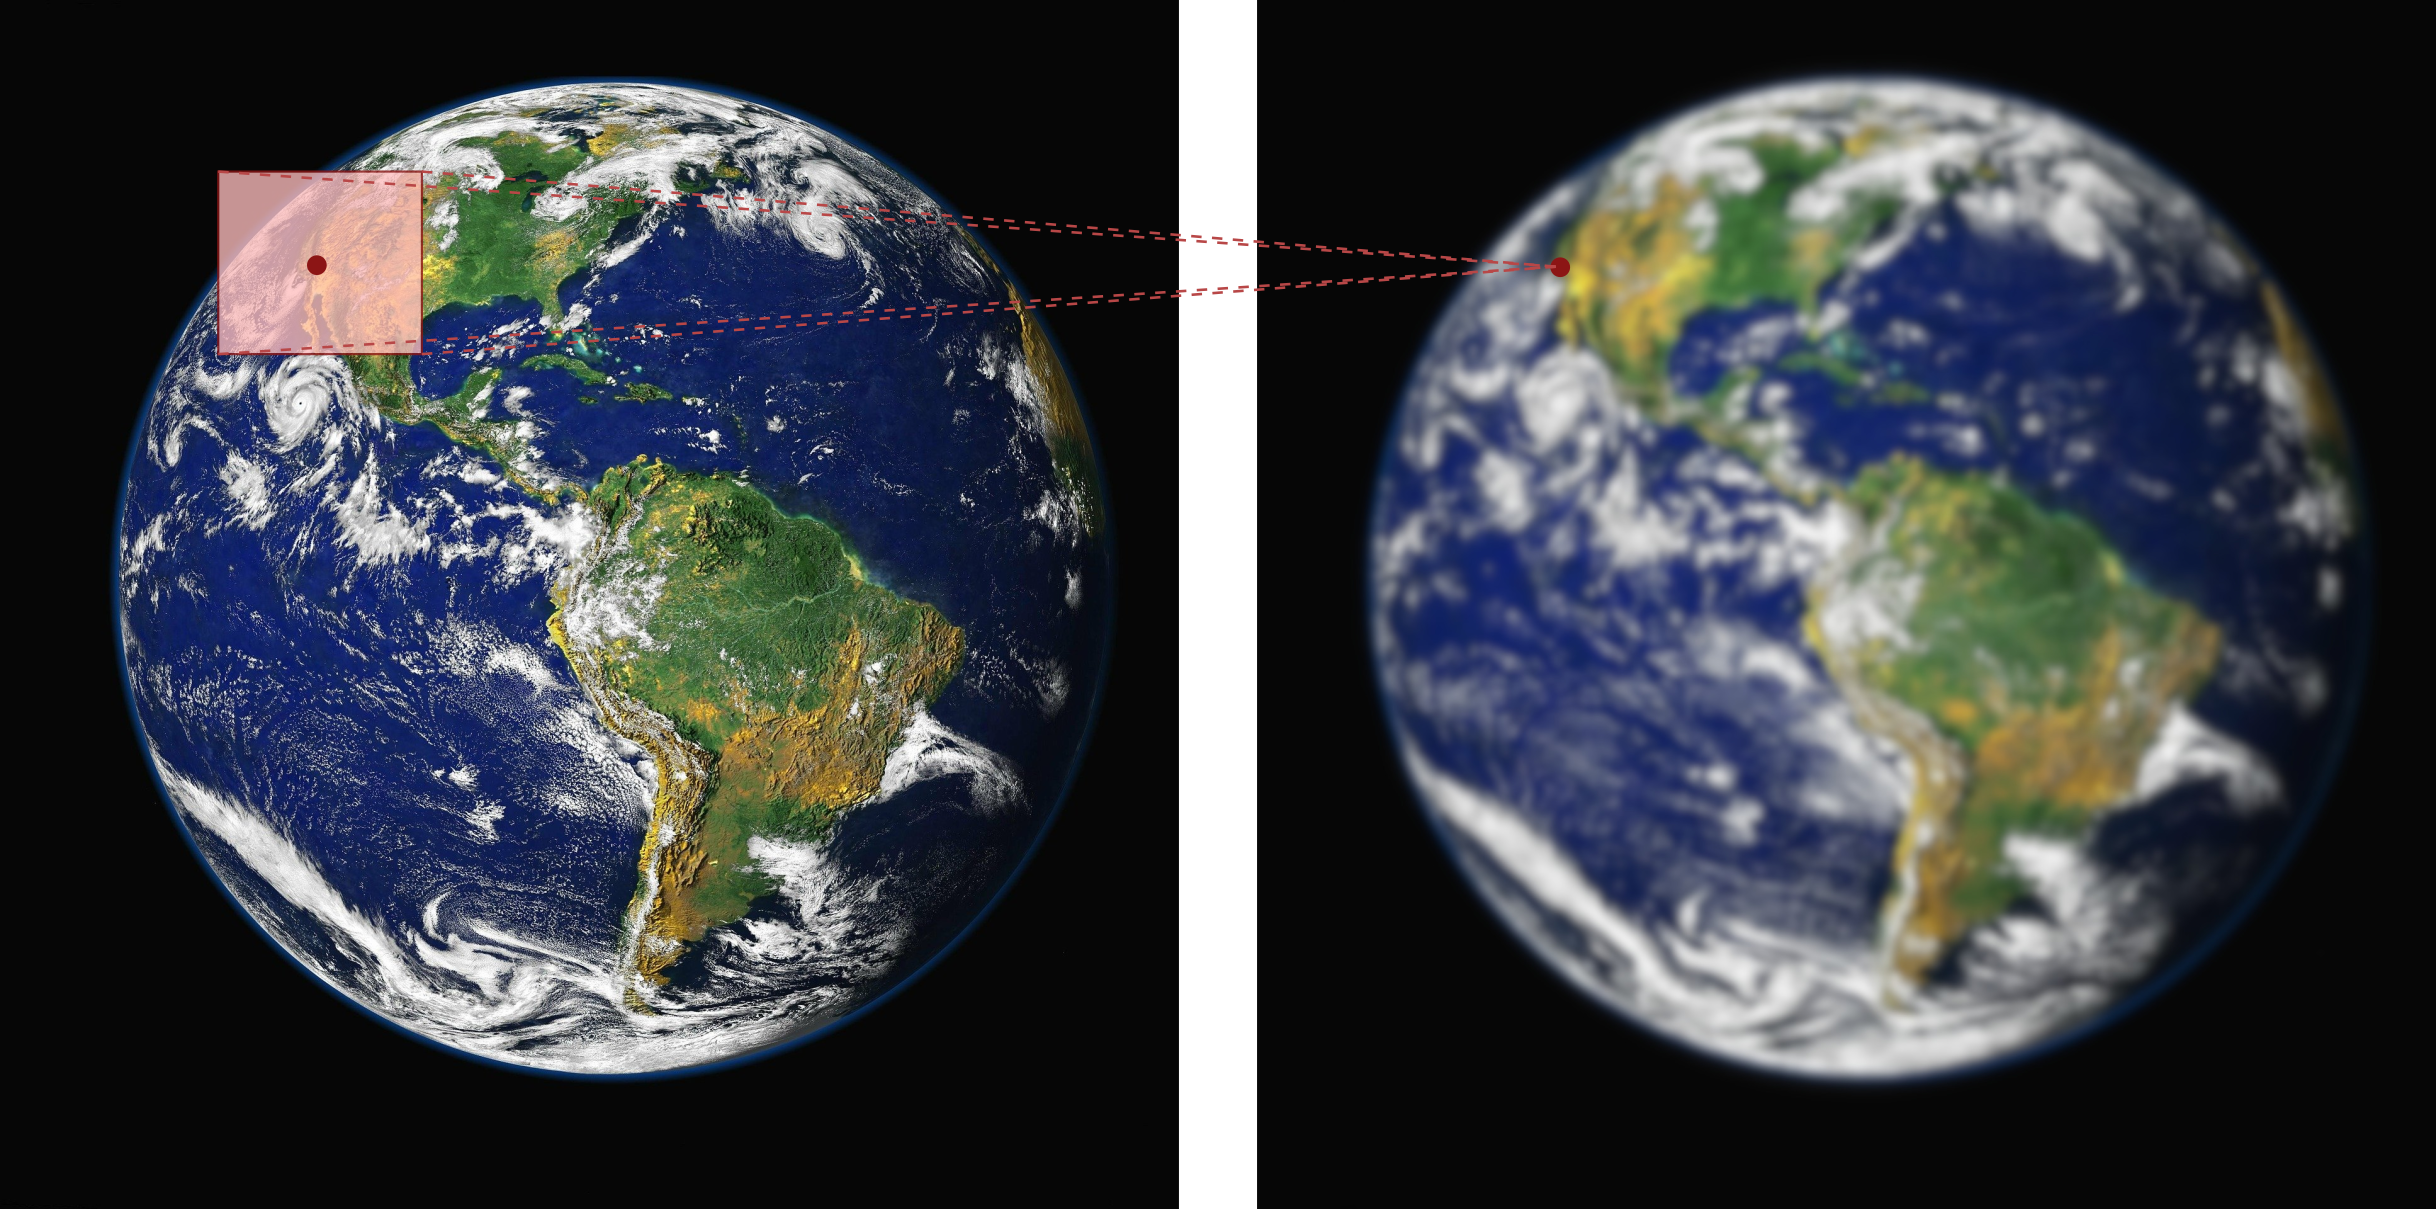
\includegraphics[width=.8\textwidth]{tex/figs/ch10_figs/gaussianfilter.png}
    \caption{Example of a Gaussian smoothing filter, which produces a smoothing (blurring) effect on the filtered image.}
    \label{fig:gaussianfilter}
\end{figure}

\subsubsection{Separable Masks}
A mask $F$ is called \textit{separable} if it can be broken down into the convolution of two kernels $F = F_1 \ast F_2$. If a mask is separable into ``smaller'' masks, then it is often cheaper to apply $F_1$ followed by $F_2$, rather than by $F$ directly. One special case of this is when the mask can be represented as an outer product of two vectors (meaning it is equivalent to the 2D convolution of those two vectors). If the mask is of shape $M\times M$, and the input image has size $w\times h$, then the computational complexity of directly performing the convolution is $O(M^2wh)$. However, by separating the masks the computational cost is $O(2Mwh)$, which is linear in $M$ rather than quadratic. As an example, consider the moving average filter mask from before: 
\begin{equation*}
F = \frac{1}{9}
\begin{bmatrix}
1 & 1 & 1\\
1 & 1 & 1\\
1 & 1 & 1
\end{bmatrix} = \frac{1}{9}
\begin{bmatrix}
1 \\
1 \\
1
\end{bmatrix}
\begin{bmatrix}
1 & 1 & 1\\
\end{bmatrix}. 
\end{equation*}
As another example, note that the Gaussian smoothing filter mask is also separable. To see why this is, note that the Gaussian weighting function can be decomposed as:
\begin{equation*}
\begin{split}
G_\sigma(x,y) &= \frac{1}{2\pi\sigma^2} \exp \bigg(-\frac{x^2 + y^2}{2\sigma^2} \bigg), \\
    &= \frac{1}{\sqrt{2\pi}\sigma}\exp \bigg(-\frac{x^2}{2\sigma^2}\bigg)\frac{1}{\sqrt{2\pi}\sigma} \exp \bigg(-\frac{y^2}{2\sigma^2}\bigg), \\
    &= g_\sigma(x) \cdot g_\sigma(y).
\end{split}
\end{equation*}

\subsubsection{Image Differentiation Filters}
Taking the derivative of an image can be used to identify certain features, such as edges. On a basic level, the derivative of an image quantifies changes in pixel intensity in both the vertical and horizontal direction. However, since images are represented as functions defined over a discrete domain the traditional method for differentiating continuous functions can not be used. Instead it is more common to just compute differences between pixels, such as using a central difference method:
\begin{equation} \label{eq:cendiff}
\begin{split}
 \frac{\partial I} {\partial x} &= \frac{I(x+1,y) - I(x-1,y)}{2},\\
\frac{\partial I} {\partial y} &= \frac{I(x,y+1) - I(x,y-1)}{2}.  
\end{split}
\end{equation}
where $\partial I/\partial x$ is the derivative in the horizontal direction and $\partial I/\partial y$ is the derivative in the vertical direction. It is of course also possible to define the derivatives using just one side, for example $\frac{\partial I}{\partial x} = I(x+1,y) - I(x,y)$.

It is also possible to differentiate an image using convolution filters. In particular, one common approach is to use a convolution filter \eqref{eq:convolution} defined with a mask $F$ called a \textit{Sobel mask} (also referred to as simply a Sobel operator). For the $x$ direction this mask is denoted as $S_x$ and for the $y$ direction as $S_y$:
\begin{equation}
S_x = \begin{bmatrix}
1 & 0 & -1\\
2 & 0 & -2\\
1 & 0 & -1
\end{bmatrix}, \quad S_y =
\begin{bmatrix}
1 & 2 & 1\\
0 & 0 & 0\\
-1 & -2 & -1
\end{bmatrix}
\end{equation}
Sobel masks are similar to the central difference method but use more neighboring pixels when calculating the derivative (i.e. they also consider the rows above and below to compute the difference). Note that Sobel masks are also separable.

\subsubsection{Similarity Measures}
Filtering can also be used to find similar features in different images, which can be useful for solving the correspondence problem in stereo vision or structure-from-motion techniques. 
In particular, the similarity between the pixel $(x,y)$ in image $I_1$ and pixel $(x', y')$ in image $I_2$ can be computed by:
\begin{equation} \label{eq:similarity}
\begin{split}
SAD &= \sum_{i=-N}^N \sum_{j=-M}^M \rvert I_1(x+i,y+j)-I_2(x^\prime+i,y^\prime+j)\lvert, \\
SSD &= \sum_{i=-N}^N \sum_{j=-M}^M [I_1(x+i,y+j)-I_2(x^\prime+i,y^\prime+j)]^2,
\end{split}
\end{equation}
where SAD is an acronym for ``sum of absolute differences'', SSD is an acronym for ``sum of squared differences'', and $N$ and $M$ define the size of the window around the pixels that is considered.

\subsection{Image Feature Detection}
A local feature (also sometimes referred to as interest points, interest regions, or keypoints) in an image is a pattern that differs from its immediate neighborhood in terms of intensity, color, or texture. 
Local features can generally be categorized in several ways, for example whether they provide semantic content or not. For example, features that may provide semantic content include edges or other geometric shapes (e.g. lanes of a road or blobs corresponding to blood cells in medical images). These types of features were some of the first for which feature detectors were proposed in the image processing literature. Features that do not provide semantic content may also be useful, for example in feature tracking, camera calibration, 3D reconstruction, image mosaicing, and panorama stitching. In these cases it may be more important that the feature be able to be located accurately and robustly over time. A third category of features are those that may not have semantic interpretations individually, but may have meaning as a collection.
For instance, a scene could be recognized by counting the number of feature matches between the observed scene and a query image. In this case only the number of matches is relevant and not the location or type of feature. Applications where these types of features are important include texture analysis, scene classification, video mining, and
image retrieval.

In this section several feature detection strategies will be discussed. While many strategies exist for different types of features, the focus here will be on two common features that are often useful in robotics: edges and corners.


\subsubsection{Edge Detection}
An \textit{edge} in an image is a region where there is a significant change in intensity values along one direction, and negligible change along the orthogonal direction. In one dimension an edge corresponds to a point where there is a sharp change in intensity, which mathematically can be thought of as a point of a function having a large first derivative and a small second derivative. Many edge detectors rely on this concept by differentiating images and looking for spikes in the derivative.
An edge detector can be evaluated based on several criteria for robustness and performance, including accuracy, localization, and single response. Good accuracy implies few false positives or negatives (missed edges), good localization implies that the detected edge should be exactly where the true edge is in the image, and a single response implies \textit{only} one edge is detected for each real edge. In practice, noise and discretization can make edge detection challenging.

Most edge detection methods rely on two key steps: smoothing and differentiation. Differentiation is performed in both the vertical and horizontal directions to find locations in the image with high intensity gradients. However, differentiation alone is vulnerable to false positives due to image noise, which is why many algorithms will first smooth the image. 

\paragraph{Edge Detection in 1D:}
An example of how noise can corrupt image differentiation is given in Figure \ref{fig:noisy}. 
\begin{figure}[ht]
  \centering
  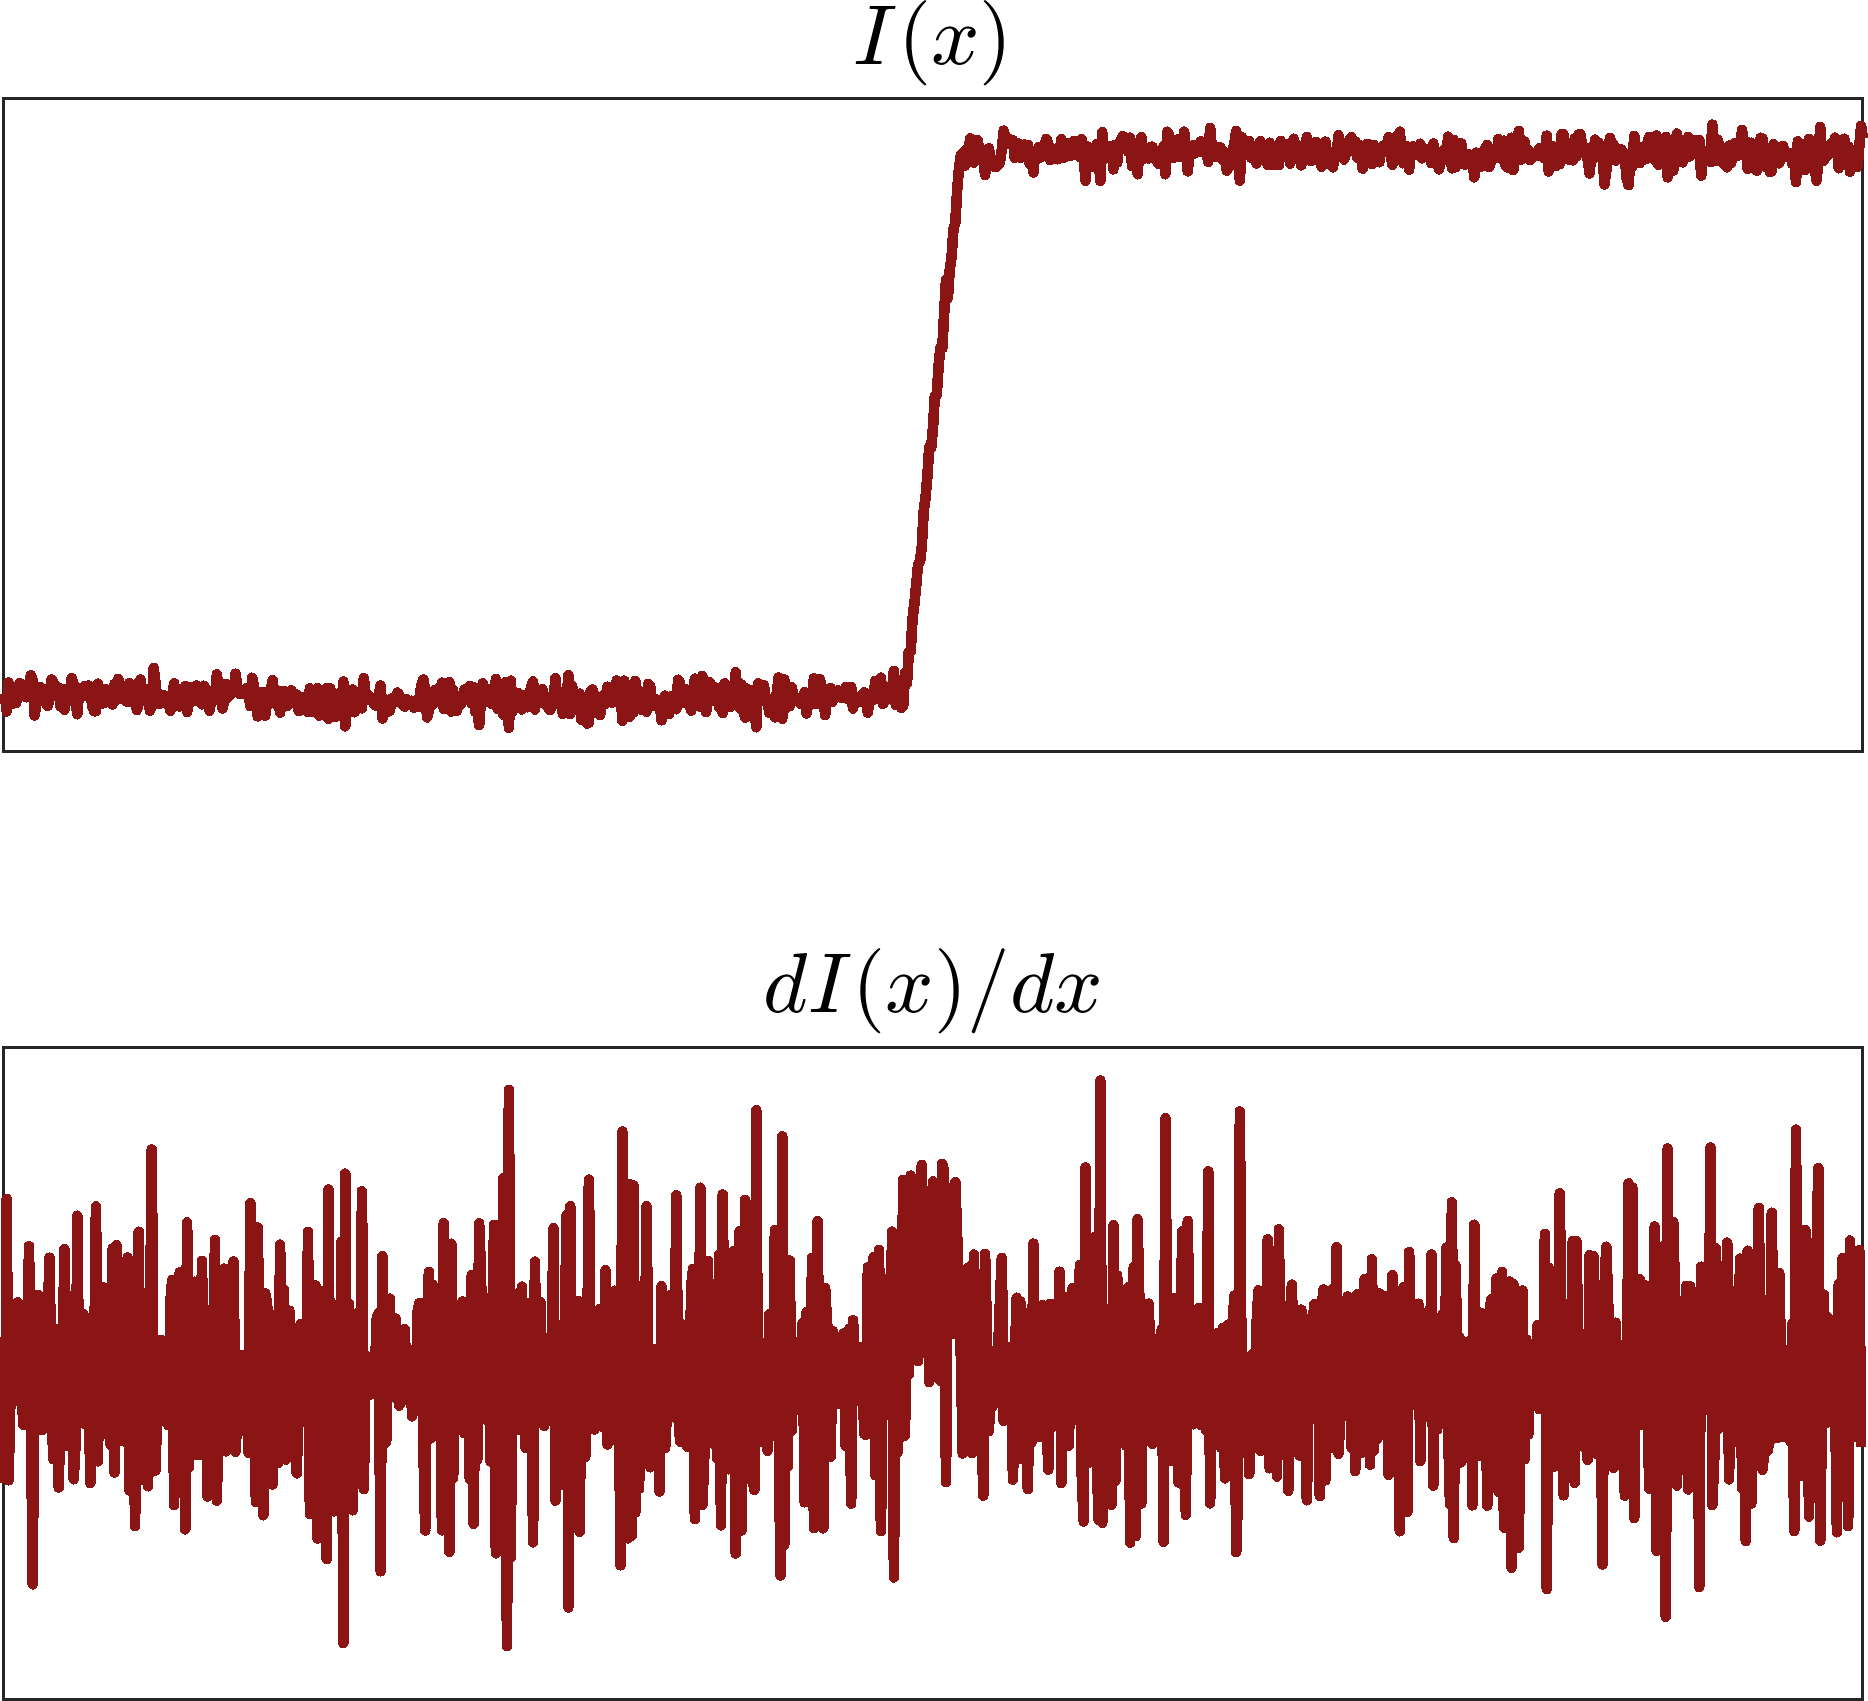
\includegraphics[width=0.5\textwidth]{tex/figs/ch10_figs/edge_detection.png}
    \caption{Differentiation of signal (e.g. for edge detection) with noise can be particularly challenging, which can be addressed by first smoothing the signal.}
    \label{fig:noisy}
\end{figure}
Notice that in this case it is impossible to identify the jump in the signal due to the noise levels.
Smoothing filters, such as the Gaussian smoothing filter discussed earlier, can help remedy this problem. In particular, suppose the original signal in Figure \ref{fig:noisy} is defined by $I(x)$. Then a smoothed version can be defined by applying a smoothing convolution filter:
\begin{equation*}
s(x) = g_\sigma(x) \ast I(x),
\end{equation*}
where $g_\sigma(x)$ represents a Gaussian smoothing filter, and then by applying the differentiation filter:
\begin{equation*}
s'(x)=\frac{d}{dx}\ast s(x).
\end{equation*}
This process is shown in Figure \ref{fig:gauss}.
\begin{figure}[ht!]
  \centering
  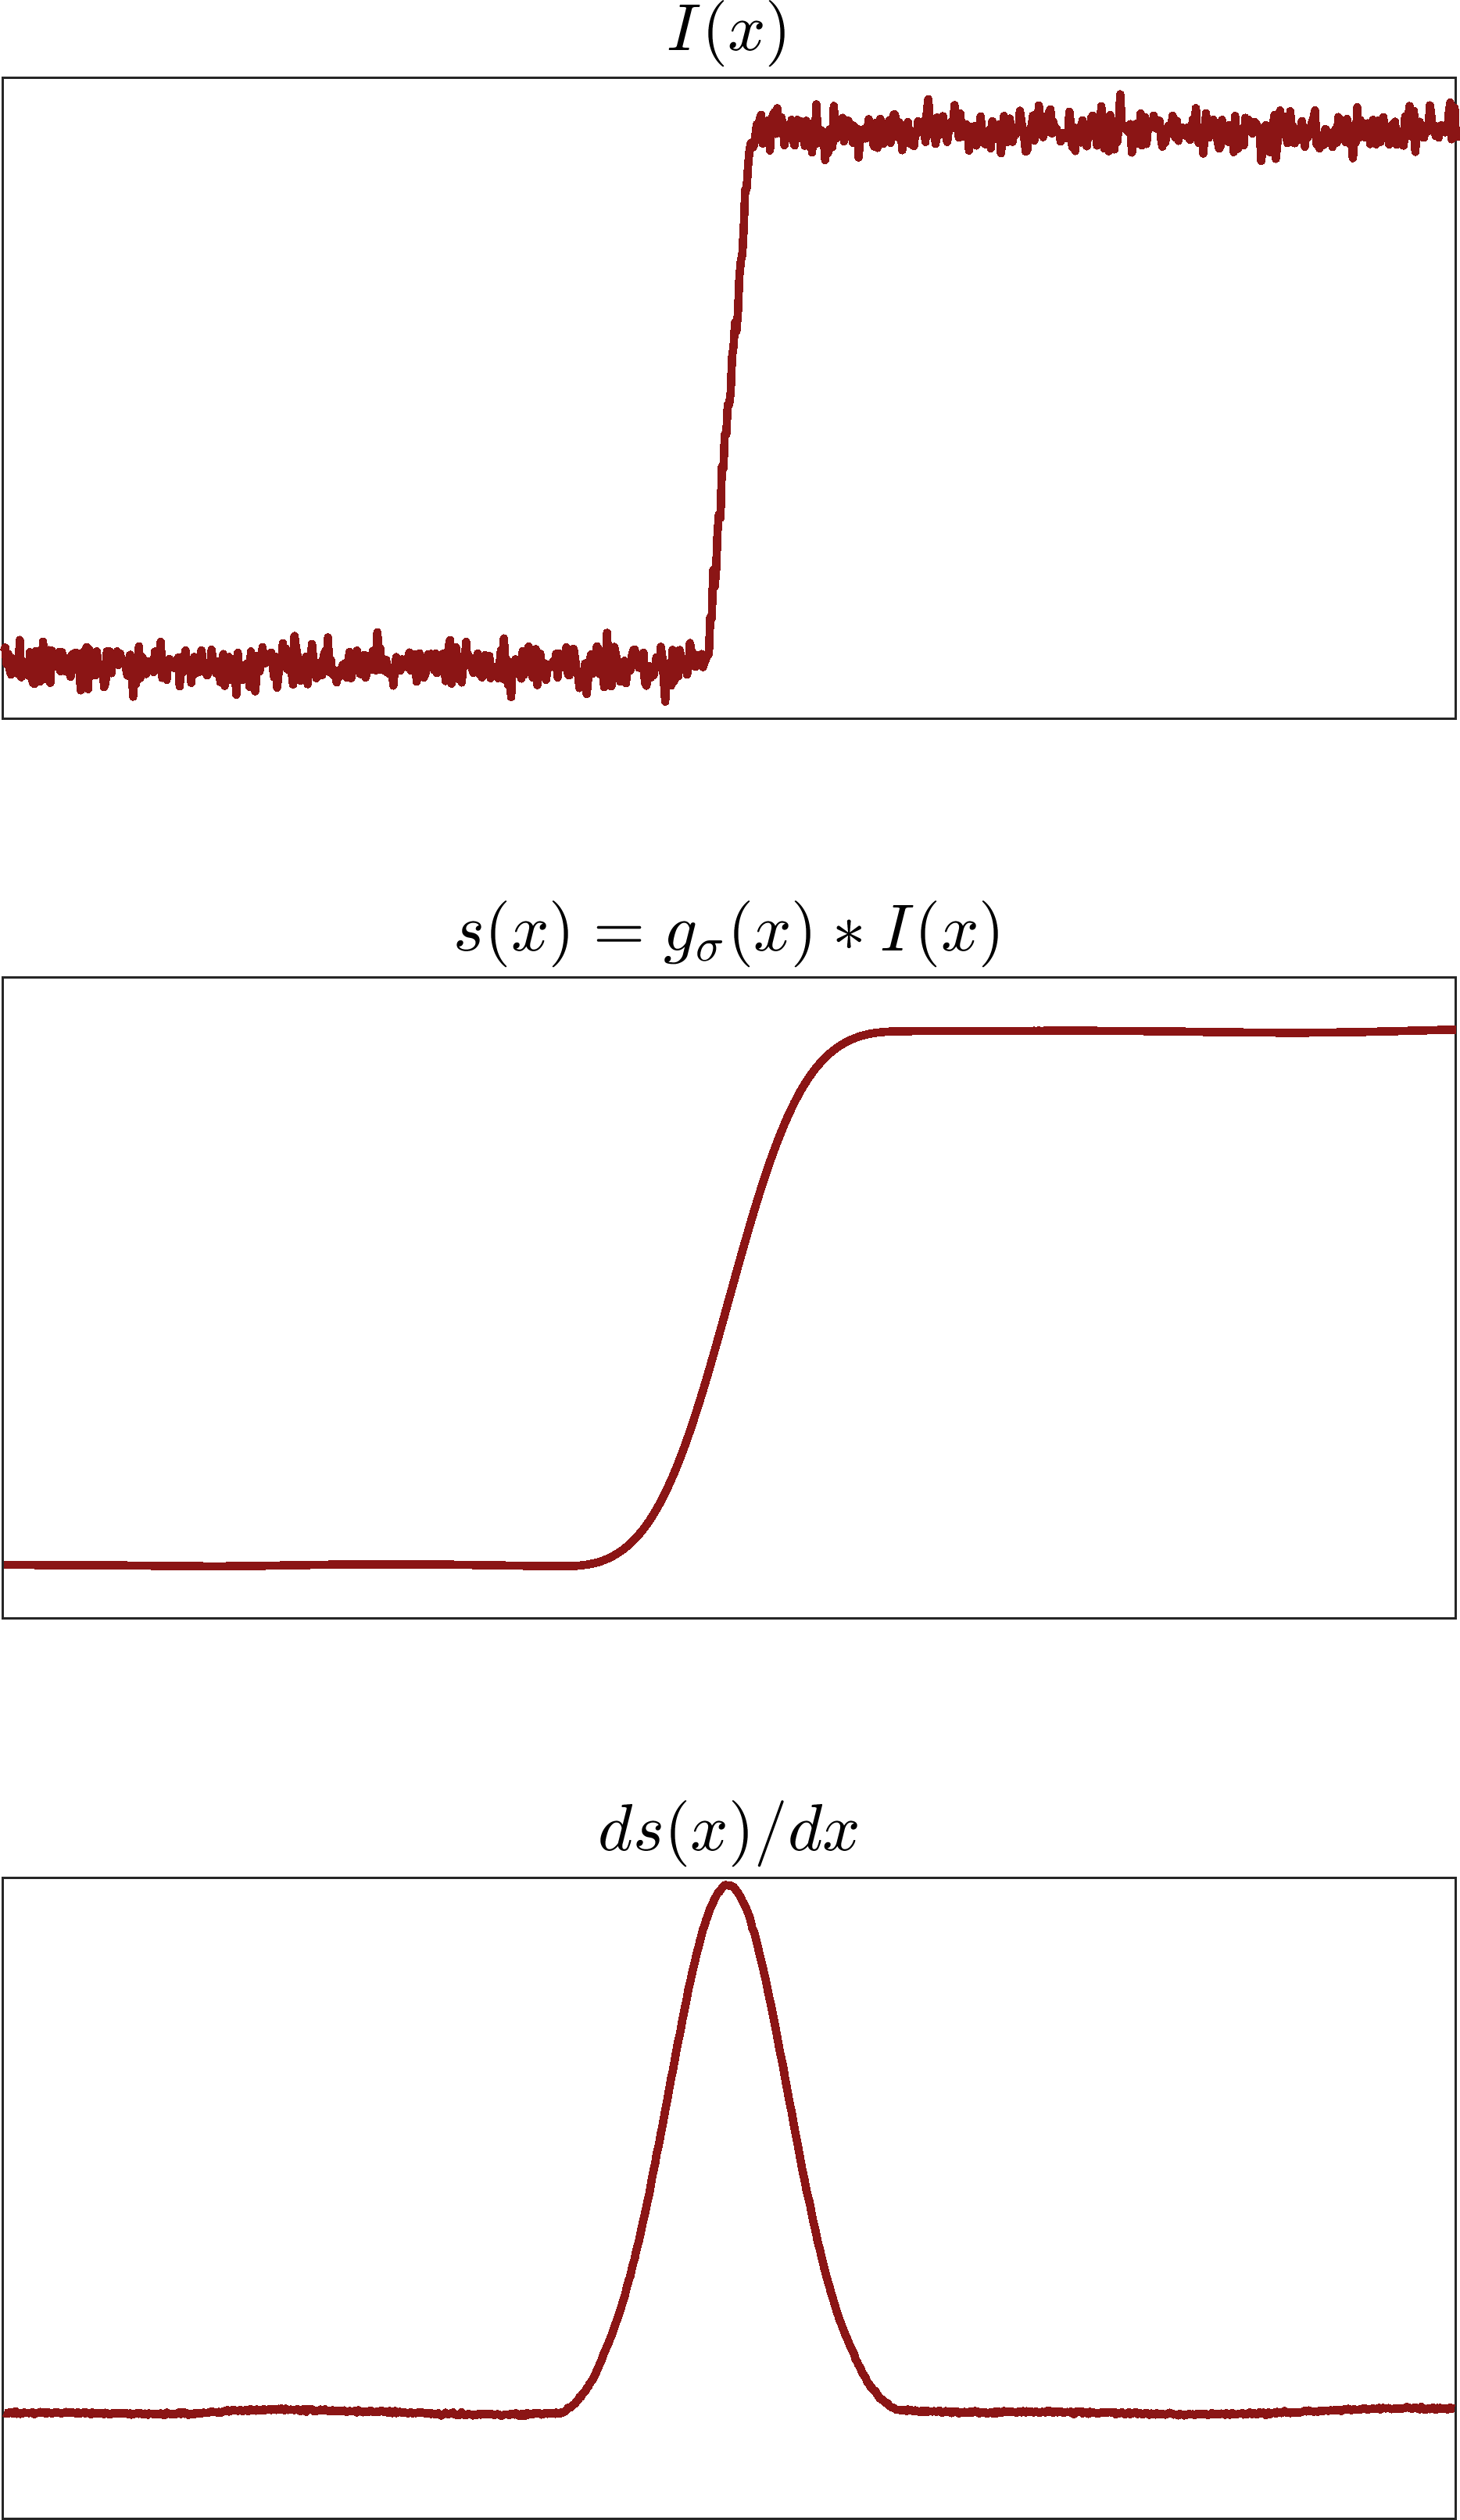
\includegraphics[width=0.55\textwidth]{tex/figs/ch10_figs/edge_detection_smooth.png}
    \caption{Edge detection through convolution with a Gaussian smoothing filter, followed by a differentiation filter.}
    \label{fig:gauss}
\end{figure}
Note however that since these filters are convolutions, the associativity property can be leveraged to actually combine them into a single filter:
\begin{equation*}
s'=(\frac{d}{dx} * g_\sigma) * I.
\end{equation*}

\paragraph{Edge Detection in 2D:}
Edge detection in a two-dimensional image is quite similar to the example previously discussed in 1D. Let the smoothing filter be the Gaussian smoothing filter from before, and a differentiation filter such as the Sobel filter. The gradient of the smoothed image in both the $x$ and $y$ directions can be written as:
\begin{equation*}
\nabla S= \begin{bmatrix}
\frac{\partial}{\partial x} * G_\sigma * I \\ \frac{\partial}{\partial y} * G_\sigma * I \end{bmatrix}= \begin{bmatrix}
G_{\sigma,x} * I\\G_{\sigma,y} * I
\end{bmatrix}=\begin{bmatrix}
S_x\\S_y
\end{bmatrix},
\end{equation*}
where $I$ is the original image and the associativity properties of the smoothing and differentiation convolution filters is used to define the combined filters $G_{\sigma,x}$ and $G_{\sigma,y}$. The magnitude of the gradient can then be computed by:
\begin{equation*}
\lvert\nabla S\rvert =\sqrt{S_x^2+S_y^2},
\end{equation*}
which can be used to check against a predefined threshold value for edge detection. To guarantee thin edges it is also possible to filter out points whose gradient magnitude are above the threshold but are not local maxima. Examples of this process are shown in Figures \ref{fig:sobel} and \ref{fig:canny}.
\begin{figure}[ht]
  \centering
  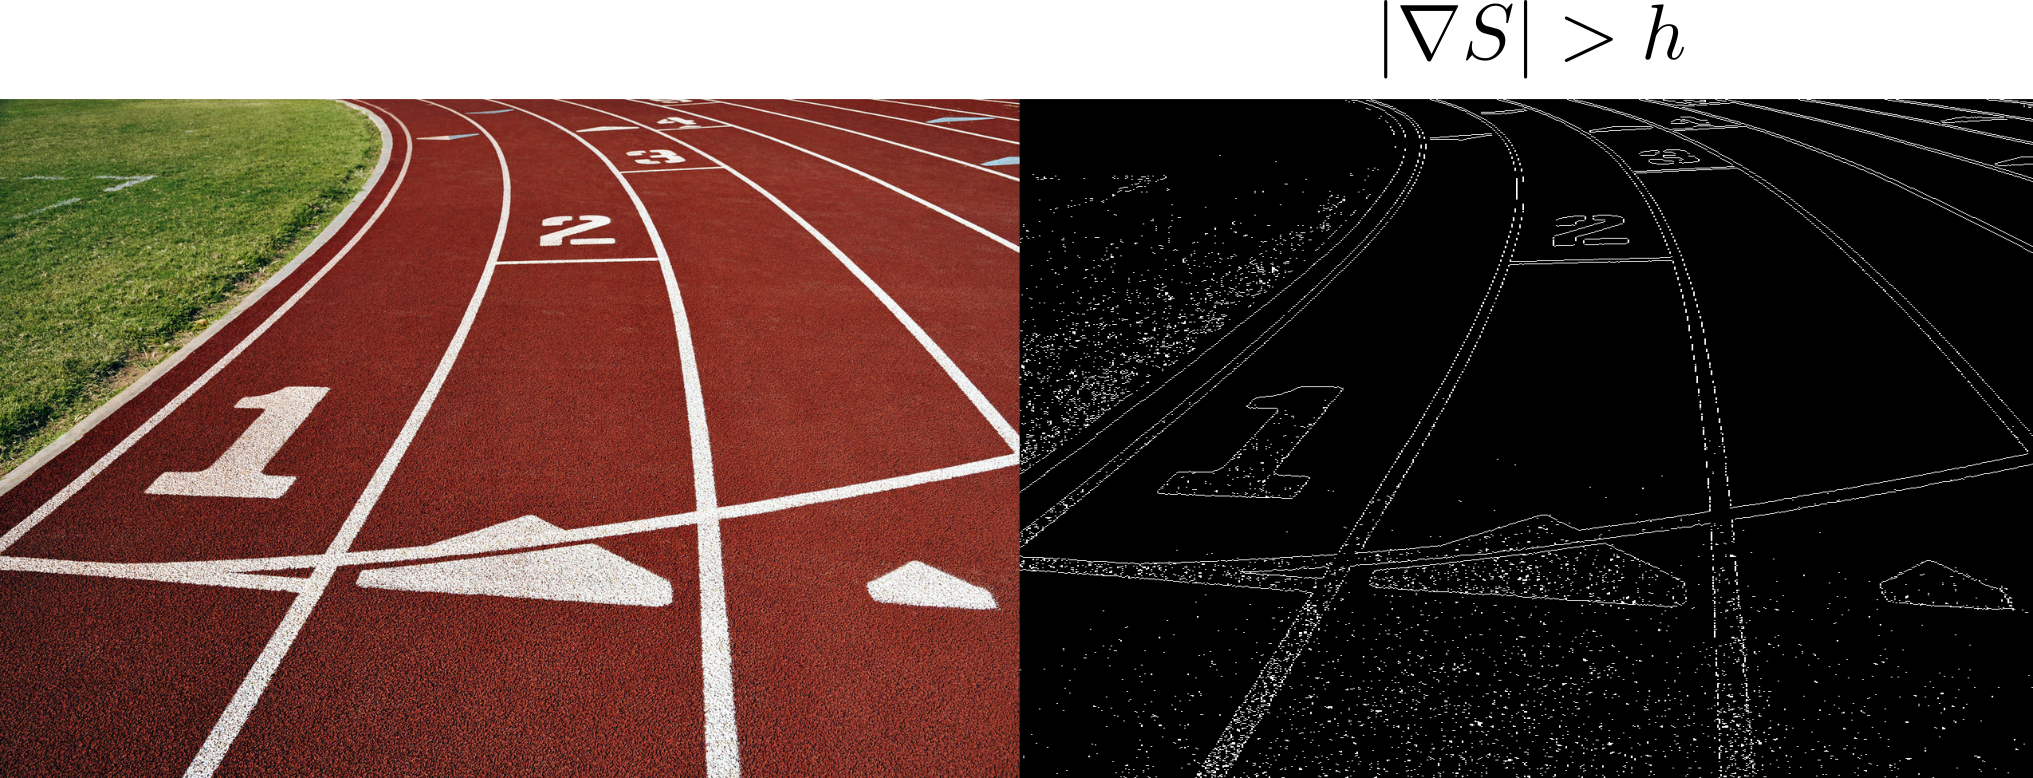
\includegraphics[width=.8\textwidth]{tex/figs/ch10_figs/sobel.png}
    \caption{Edge detection using the ``Sobel'' edge detector.}
    \label{fig:sobel}
\end{figure}
\begin{figure}[ht]
  \centering
  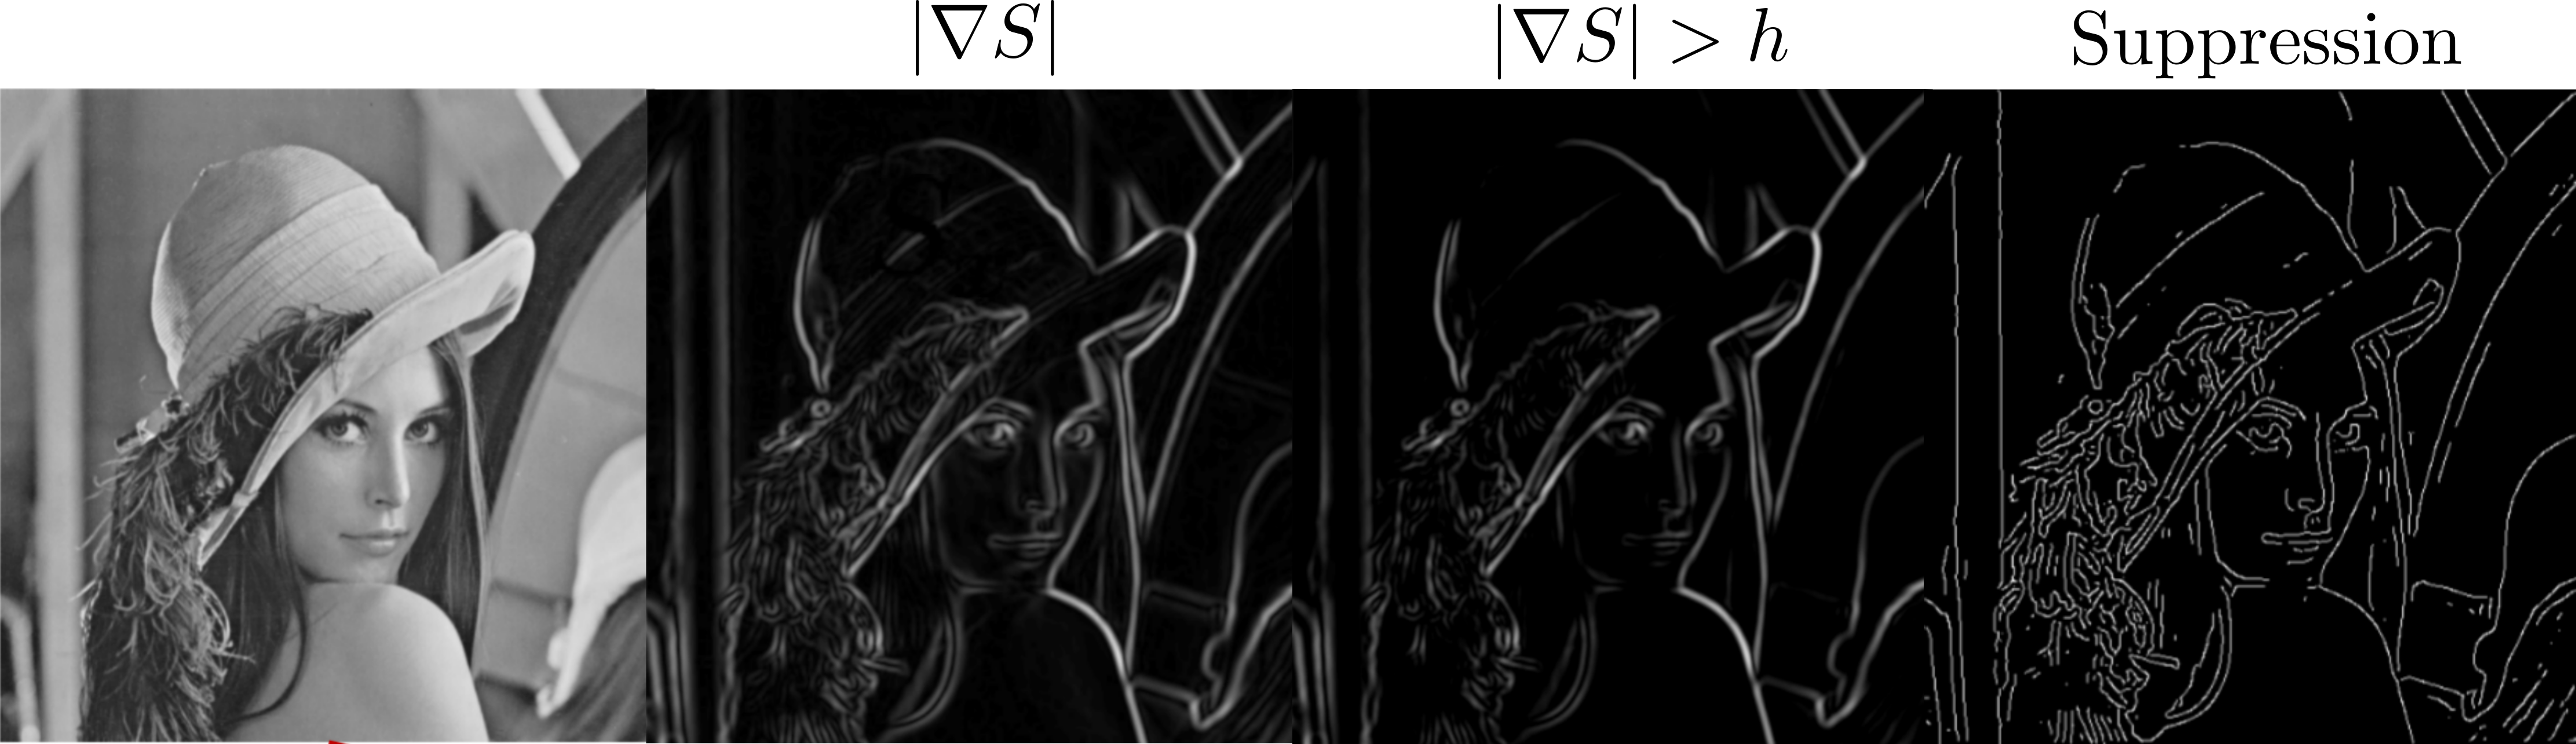
\includegraphics[width=.8\textwidth]{tex/figs/ch10_figs/canny.png}
    \caption{Edge detection using the ``Canny'' edge detector.}
    \label{fig:canny}
\end{figure}

\subsubsection{Corner Detection}
A \textit{corner} in an image is defined as an intersection of two or more edges, and also sometimes as a point where there is a large intensity variation in every direction. 
Important properties of corner detectors include repeatability and distinctiveness. Repeatability quantifies how well the same features can be found in multiple images even under geometric and photometric transformations. Distinctiveness refers to whether the information carried by the patch surrounding the feature is distinctive, which can be used to reliably produce correspondences. Both of these properties are particularly important in applications such as panorama stitching and 3D reconstruction.

Generally corner detection can be thought of in a similar way to edge detection, except that instead of looking for change along one direction there should be changes in all directions. One well known corner detector is known as the Harris detector \cite{Harris1988}, which has the useful property that the detection is invariant to rotations and linear intensity changes (i.e. geometric and photometric invariance). However the Harris detector is not invariant to scale changes or geometric affine changes, which has led to the development of scale-invariant detectors such as the Harris-Laplacian detector or the scale-invariant feature transform (SIFT) detector.

\subsection{Image Descriptors}
Image \textit{descriptors} describe features so that they can be compared across images, or used for object detection and matching. Similar to image detectors, it is also desirable for image descriptors to be repeatable (i.e. invariant with respect to pose, scale, illumination, etc.) and distinct. Perhaps the simplest example of a descriptor is an $n\times m$ window of pixel intensities centered at the feature, which can be normalized to be illumination invariant. However, such a descriptor is not invariant to pose or scale and is not distinctive, and therefore is generally not useful in practice. 
Alternative detectors/descriptors that have become popular include SIFT, SURF, FAST, BRIEF, ORB, and BRISK. 

\subsection{Exercises}
\subsubsection{Linear Filtering}
Complete \textit{Problem 3: Linear Filtering} located in the online repository:

\vspace{\baselineskip}

\url{https://github.com/PrinciplesofRobotAutonomy/AA274A_HW3},

\vspace{\baselineskip}

where you will explore the use of linear filters for image processing.